\documentclass[11pt]{article}

% ---------------------------------------------------------------------------
%  OncoEvidence -- SRI / OpenBio Research Proposal (basic plan for mentor)
%  Compile with:  tectonic docs/proposal.tex
% ---------------------------------------------------------------------------

\usepackage[margin=1in]{geometry}
\usepackage{amsmath,amssymb}
\usepackage{xcolor}
\usepackage{tikz}
\usetikzlibrary{arrows.meta,positioning,fit,backgrounds,calc,shapes.geometric}
\usepackage{booktabs}
\usepackage{array}
\usepackage{colortbl}
\usepackage[most]{tcolorbox}
\usepackage{enumitem}
\usepackage{graphicx}
\usepackage{float}

% ----- Palette -------------------------------------------------------------
\definecolor{sriblue}{HTML}{1F4E79}
\definecolor{sriaccent}{HTML}{E8684A}
\definecolor{srigreen}{HTML}{2E8B57}
\definecolor{srigray}{HTML}{4B5563}
\definecolor{srilight}{HTML}{EAF1F8}
\definecolor{sriamber}{HTML}{F6BD16}
\definecolor{srirow}{HTML}{F2F6FB}
\definecolor{nDrug}{HTML}{E8684A}
\definecolor{nDis}{HTML}{5B8FF9}
\definecolor{nGene}{HTML}{2E8B57}
\definecolor{nPath}{HTML}{F6BD16}

\usepackage[colorlinks=true,linkcolor=sriblue,citecolor=sriblue,urlcolor=sriaccent]{hyperref}

\usepackage{titlesec}
\titleformat{\section}{\large\bfseries\color{sriblue}}{\thesection}{0.6em}{}
\titleformat{\subsection}{\normalsize\bfseries\color{sriblue!85!black}}{\thesubsection}{0.5em}{}
\titlespacing*{\section}{0pt}{1.4ex}{0.8ex}

\newtcolorbox{problembox}{colback=srilight,colframe=sriblue,boxrule=0.9pt,
  arc=2pt,left=6pt,right=6pt,top=5pt,bottom=5pt}
\newtcolorbox{aimbox}[1]{colback=srigreen!7,colframe=srigreen,boxrule=0.8pt,
  arc=2pt,left=6pt,right=6pt,top=4pt,bottom=4pt,title={#1},
  fonttitle=\bfseries\color{white},colbacktitle=srigreen}

\renewcommand{\arraystretch}{1.25}
\newcommand{\NN}{\mathcal{N}}

\begin{document}

\begin{center}
  {\LARGE\bfseries\color{sriblue} OncoEvidence: Mechanism-Guided Evidence\\ Triage for Cancer Drug Repurposing}\\[4pt]
  {\large\bfseries\color{sriblue!80!black} A knowledge-graph and language-model pipeline that prioritizes\\ repurposing candidates by mechanistic plausibility and literature evidence}\\[10pt]
  {\large Akshatha Arunkumar}\\[2pt]
  {\small Student Research Institute (SRI), Summer 2026 Cohort \\
  Harvard Undergraduate OpenBio Laboratory}\\[2pt]
  {\small\itshape Research Proposal for Mentor Review \quad\textbar\quad \today}
\end{center}

\vspace{2pt}
\begin{problembox}
\textbf{The problem.} Drug repurposing looks for new uses of existing drugs, for
example asking whether an approved drug could treat a cancer it was not designed
for. Computational methods can rank thousands of drug-disease pairs, but a high
score is not enough: a researcher still needs to know \emph{why} a drug might work
(its mechanism) and whether the literature supports it. This project builds a
pipeline that, for cancer repurposing, ranks candidates, extracts the biological
mechanism path that would explain each one, and checks that mechanism against
published evidence.
\end{problembox}

\begin{aimbox}{Proposed study}
I will build an oncology-focused evidence-triage pipeline on the PrimeKG
biomedical knowledge graph. It will (1) rank drug-cancer candidates and compare a
graph model against a strong tabular baseline to test honestly when the graph
helps, (2) extract multi-hop \emph{drug $\rightarrow$ target protein $\rightarrow$
cancer gene $\rightarrow$ cancer} mechanism paths for the top candidates, and
(3) use a language model to read the literature and grade whether each mechanism
is supported. I will evaluate the system against known indications and a curated
mechanism database. The deliverable is a ranked, evidence-backed shortlist of
repurposing candidates with transparent mechanistic rationales.
\end{aimbox}

\vspace{4pt}
\noindent\textit{Why this project.} I am drawn to drug repurposing because it can
bring existing, already-safe drugs to new cancer patients faster than designing a
drug from scratch. What interests me technically is the gap between a prediction
and an explanation: a model can output a score, but a clinician or scientist needs
a reason. I want to build a system that produces the reason and then checks it
against the evidence.

% ===========================================================================
\section{Background and Significance}

Cancer drug repurposing matters because developing a new drug takes many years and
large cost, while thousands of approved drugs already have known safety profiles.
If one of them acts on a protein or pathway that also drives a cancer, it may be a
fast route to a new treatment. Biomedical knowledge graphs such as PrimeKG collect
millions of relationships among drugs, proteins, genes, pathways, and diseases, so
the information needed to reason about such mechanisms is, in principle, already
encoded as paths through the graph.

The challenge is trust. A model that only outputs a drug-disease score is hard to
act on, because the reviewer cannot see the reasoning and cannot tell a real
mechanism from a coincidence. Recent work has shown that graph models can predict
repurposing links and even suggest paths, and that language models can reason over
biomedical text. What is still under-explored is an honest, evaluated combination:
a system that produces a mechanism and then verifies it against the literature,
and that reports clearly when the graph is actually necessary.

% ===========================================================================
\section{Central Question and Specific Aims}

\begin{problembox}
\textbf{Core question.} For cancer drug repurposing, can we separate \emph{ranking}
from \emph{justification}, using a strong non-graph ranker to prioritize candidates
while using a biomedical knowledge graph and a literature-grounded language model to
extract, audit, and score the mechanism behind each one, and what does the graph add
once a tuned tabular ranker is already in place?
\end{problembox}

\begin{aimbox}{Specific Aims}
\textbf{Aim 1 (Candidate generation with calibrated baselines).} Use a tuned
XGBoost as the primary ranker, and treat a heterogeneous graph network and a
knowledge-graph embedding as ablations, measuring whether graph message passing
improves ranking under leakage-safe transductive and inductive splits.\\
\textbf{Aim 2 (Mechanism extraction, the graph's real role).} The graph is the
mechanism engine, not the ranker. For top candidates, extract multi-hop
\emph{drug $\rightarrow$ target $\rightarrow$ pathway/cancer-gene $\rightarrow$
cancer} paths, prioritizing real mechanism relations over phenotype coincidence.\\
\textbf{Aim 3 (Evidence verification).} Retrieve literature and have a language
model grade each path as supported, weak, contradicted, or unknown, with a quoted
piece of evidence.\\
\textbf{Aim 4 (Evaluation).} Test the system against known indications and a
curated mechanism resource (DrugMechDB), measuring whether mechanism paths
separate true indications from random pairs and whether verified mechanisms agree
with curated ones.
\end{aimbox}

% ===========================================================================
\section{Datasets}

\begin{table}[H]
\centering\small
\begin{tabular}{>{\raggedright\arraybackslash}p{0.26\linewidth} >{\raggedright\arraybackslash}p{0.42\linewidth} >{\raggedright\arraybackslash}p{0.24\linewidth}}
\toprule
\rowcolor{sriblue}\color{white}\textbf{Resource} & \color{white}\textbf{Content} & \color{white}\textbf{Role}\\
\midrule
\rowcolor{srirow} PrimeKG & biomedical knowledge graph: drugs, proteins, genes, pathways, diseases ($\sim$129k nodes, $\sim$8M edges) & Candidate ranking + mechanism paths\\
Europe PMC & open biomedical literature API (titles, abstracts, open-access full text) & Evidence retrieval for verification\\
\rowcolor{srirow} DrugMechDB & expert-curated drug mechanism-of-action paths & Ground truth for mechanism evaluation\\
\bottomrule
\end{tabular}
\caption{All resources are public. PrimeKG supplies the graph; Europe PMC supplies
the evidence; DrugMechDB supplies curated mechanisms to evaluate against.}
\label{tab:data}
\end{table}

% ===========================================================================
\section{Proposed Methodology}

\textbf{Knowledge graph and candidate ranking.} I will represent PrimeKG as a
heterogeneous graph and frame repurposing as link prediction on the
\emph{drug $\rightarrow$ indication $\rightarrow$ disease} edges: hide some known
treatment links and score drug-disease pairs that are not currently connected. I
will give the graph model and the tabular baseline the \emph{same} node features
(text embeddings of names and descriptions), so any difference measures the value
of graph structure rather than the features.

\textbf{Mechanism extraction.} For top-ranked candidates I will search the graph
for short, specific paths connecting a drug to a cancer through its target protein,
protein interactions, and shared pathways, while down-weighting generic hub
proteins (such as common drug carriers) so the paths stay mechanistic.

\textbf{Evidence verification.} For each mechanism path I will retrieve relevant
abstracts from Europe PMC and ask a language model to decide whether the text
supports that specific mechanism, requiring it to quote the supporting sentence and
to treat a mere statistical association as weak rather than supporting evidence.

\begin{figure}[H]
\centering
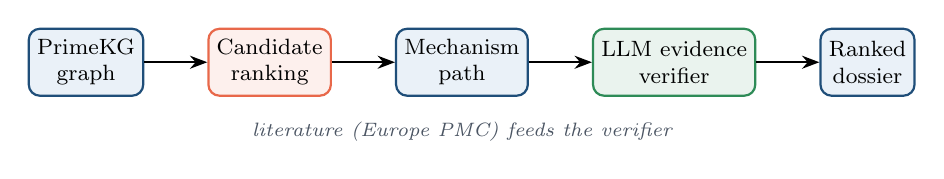
\begin{tikzpicture}[
  node distance=6mm and 8mm,
  box/.style={rounded corners,draw=sriblue,fill=srilight,thick,align=center,font=\footnotesize,inner sep=3pt,minimum height=0.85cm},
  acc/.style={rounded corners,draw=sriaccent,fill=sriaccent!10,thick,align=center,font=\footnotesize,inner sep=3pt,minimum height=0.85cm},
  grn/.style={rounded corners,draw=srigreen,fill=srigreen!10,thick,align=center,font=\footnotesize,inner sep=3pt,minimum height=0.85cm},
  >={Stealth[length=2.2mm]}]
  \node[box] (kg) {PrimeKG\\graph};
  \node[acc,right=of kg] (rank) {Candidate\\ranking};
  \node[box,right=of rank] (mech) {Mechanism\\path};
  \node[grn,right=of mech] (llm) {LLM evidence\\verifier};
  \node[box,right=of llm] (out) {Ranked\\dossier};
  \draw[->,thick] (kg)--(rank); \draw[->,thick] (rank)--(mech);
  \draw[->,thick] (mech)--(llm); \draw[->,thick] (llm)--(out);
  \node[srigray,font=\scriptsize\itshape,below=2mm of mech] {literature (Europe PMC) feeds the verifier};
\end{tikzpicture}
\caption{Planned pipeline: rank candidates on the graph, extract a mechanism path
for each, verify the path against the literature, and output an evidence-backed
shortlist.}
\label{fig:pipeline}
\end{figure}

% ===========================================================================
\section{Planned Evaluation}

I will not rely on a single accuracy number. The plan is to test the system from
several angles (Table~\ref{tab:eval}), with an emphasis on whether the mechanisms
are real, not just whether the scores are high.

\begin{table}[H]
\centering\small
\begin{tabular}{>{\raggedright\arraybackslash}p{0.30\linewidth} >{\raggedright\arraybackslash}p{0.62\linewidth}}
\toprule
\rowcolor{sriblue}\color{white}\textbf{Question} & \color{white}\textbf{How I will test it}\\
\midrule
\rowcolor{srirow} Is the graph necessary for ranking? & Graph model vs tuned XGBoost on the same features, under leakage-safe splits.\\
Do mechanism paths mean anything? & Do true indications carry stronger mechanism paths than \emph{degree-matched and same-area hard negatives} (not just random pairs)?\\
\rowcolor{srirow} Are the mechanisms real? & Agreement of extracted paths with curated DrugMechDB mechanisms (gene- and path-level).\\
Is the evidence verification trustworthy? & Precision of ``supported'' calls vs curated mechanisms, with confidence intervals and leakage controls.\\
\bottomrule
\end{tabular}
\caption{Planned evaluation. The goal is an honest picture of where the system
works, including reporting any place where a simple baseline is already enough.}
\label{tab:eval}
\end{table}

% ===========================================================================
\section{Relationship to Prior Work}

This project does not claim to invent knowledge-graph or language-model drug
repurposing; close prior work exists and I treat it as reference. TxGNN (Nature
Medicine, 2024) is a graph model for zero-shot repurposing with multi-hop
explanations; KGML-xDTD predicts treatment links with mechanism paths; DrugKLM
combines knowledge graphs with language-model reasoning; and Decagon showed graph
models excel on relational drug-pair tasks. My contribution is narrower and honest:
an oncology-specific, literature-grounded evidence-triage pipeline that tests when
the graph is actually necessary and evaluates whether the proposed mechanisms are
supported by retrieved literature and curated databases. I combine and evaluate; I
do not claim to be first.

% ===========================================================================
\section{Eight-Week Timeline}

\begin{table}[H]
\centering\small
\begin{tabular}{>{\raggedright\arraybackslash}p{0.14\linewidth} >{\raggedright\arraybackslash}p{0.78\linewidth}}
\toprule
\rowcolor{sriblue}\color{white}\textbf{Weeks} & \color{white}\textbf{Milestones}\\
\midrule
\rowcolor{srirow} 1--2 & Build the PrimeKG pipeline; set up leakage-safe splits and shared features.\\
3--4 & Candidate ranking (graph model, knowledge-graph embedding) and the tuned XGBoost baseline.\\
\rowcolor{srirow} 5 & Mechanism-path extraction with hub down-weighting; sanity-check on known drugs.\\
6 & Literature retrieval and the language-model verifier (supported/weak/contradicted/unknown).\\
\rowcolor{srirow} 7 & Evaluation: separation test, DrugMechDB agreement, verifier precision.\\
8 & Deliverable shortlist, figures, and a written report.\\
\bottomrule
\end{tabular}
\caption{Schedule for the eight-week SRI cohort.}
\label{tab:timeline}
\end{table}

% ===========================================================================
\section{Reproducibility and Ethics}

I will use open tools (PyTorch Geometric, scikit-learn, XGBoost) and public data
(PrimeKG, Europe PMC, DrugMechDB), and will release code, configurations, and
random seeds. All predictions are research-only and hypothesis-generating; they are
not medical advice and would require experimental and clinical validation before any
use.

% ===========================================================================
\begin{thebibliography}{9}
\small
\bibitem{txgnn} Huang K, Chandak P, et al. \textit{A foundation model for
clinician-centered drug repurposing (TxGNN)}. Nature Medicine, 2024.
\bibitem{primekg} Chandak P, Huang K, Zitnik M. \textit{Building a knowledge graph
to enable precision medicine (PrimeKG)}. Scientific Data, 2023.
\bibitem{kgmlxdtd} \textit{KGML-xDTD: a knowledge graph-based framework for drug
treatment prediction and mechanism description}. 2023.
\bibitem{decagon} Zitnik M, Agrawal M, Leskovec J. \textit{Modeling polypharmacy
side effects with graph convolutional networks (Decagon)}. Bioinformatics, 2018.
\bibitem{drugmechdb} Mayers M, et al. \textit{DrugMechDB: a curated database of
drug mechanism paths}. 2022.
\end{thebibliography}

\end{document}
